\documentclass[12pt]{article}

\usepackage{fixltx2e}
\usepackage{textcomp}
\usepackage{fullpage}
\usepackage{amsfonts}
\usepackage{verbatim}
\usepackage[english]{babel}
\usepackage{pifont}
\usepackage{color}
\usepackage{setspace}
\usepackage{lscape}
\usepackage{indentfirst}
\usepackage[normalem]{ulem}
\usepackage{booktabs}
% \usepackage{nag}
\usepackage{natbib}
% \usepackage{bibtex}
\usepackage{float}
\usepackage{latexsym}
\usepackage{hyperref}
\usepackage{url}
% \usepackage{html}
\usepackage{epsfig}
\usepackage{graphicx}
\usepackage{amssymb}
\usepackage{amsmath}
\usepackage{bm}
\usepackage{array}
%\usepackage{mhchem}
\usepackage{ifthen}
\usepackage{caption}
\usepackage{xcolor}
\usepackage{amsthm}
\usepackage{amstext}
\usepackage{nicefrac}
\usepackage{algorithm}
\usepackage{algorithmic}
\usepackage[scientific-notation=true]{siunitx}
\usepackage{subfigure}
\usepackage[flushleft]{threeparttable}
\usepackage{lineno}
\usepackage{adjustbox}

%Rename figure or table label number
\renewcommand{\thefigure}{S\arabic{figure}}
\renewcommand{\thetable}{S\arabic{table}}

\begin{document}

\begin{minipage}[h]{\textwidth}
	\title{Supplementary information for StarBEAST2}
	\author{Huw A. Ogilvie$^{\ast,1,2}$ and Alexei J. Drummond,$^{2,3}$}
    \maketitle
\end{minipage}

\raggedright
$^{1}$Department of Evolution, Ecology and Genetics, Australian National University, Canberra, Australia\\
$^{2}$Centre for Computational Evolution, University of Auckland, Auckland, New Zealand\\
$^{3}$Department of Computer Science, University of Auckland, Auckland, New Zealand

\clearpage

\section{Validation of correctness}

\begin{figure}[htb!]
\centering
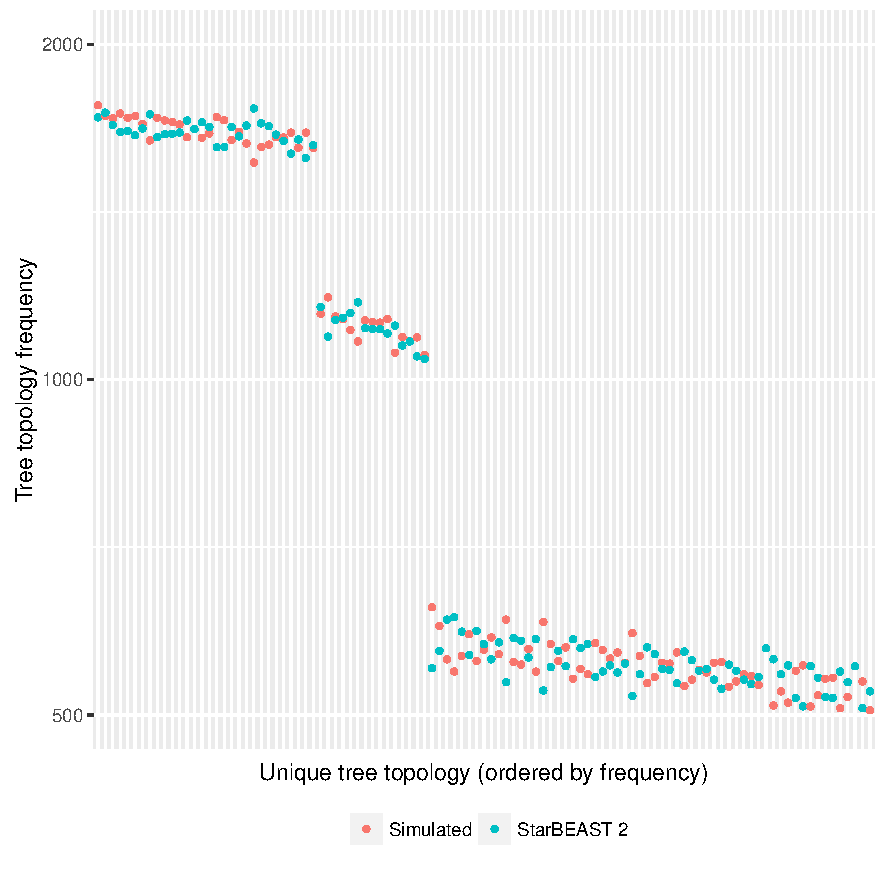
\includegraphics[width=16cm]{species_topology_frequencies.pdf}
\caption
{aaa.}
\label{fig:speciesTopologyFrequencies}
\end{figure}

\clearpage

\begin{figure}[htb!]
\centering
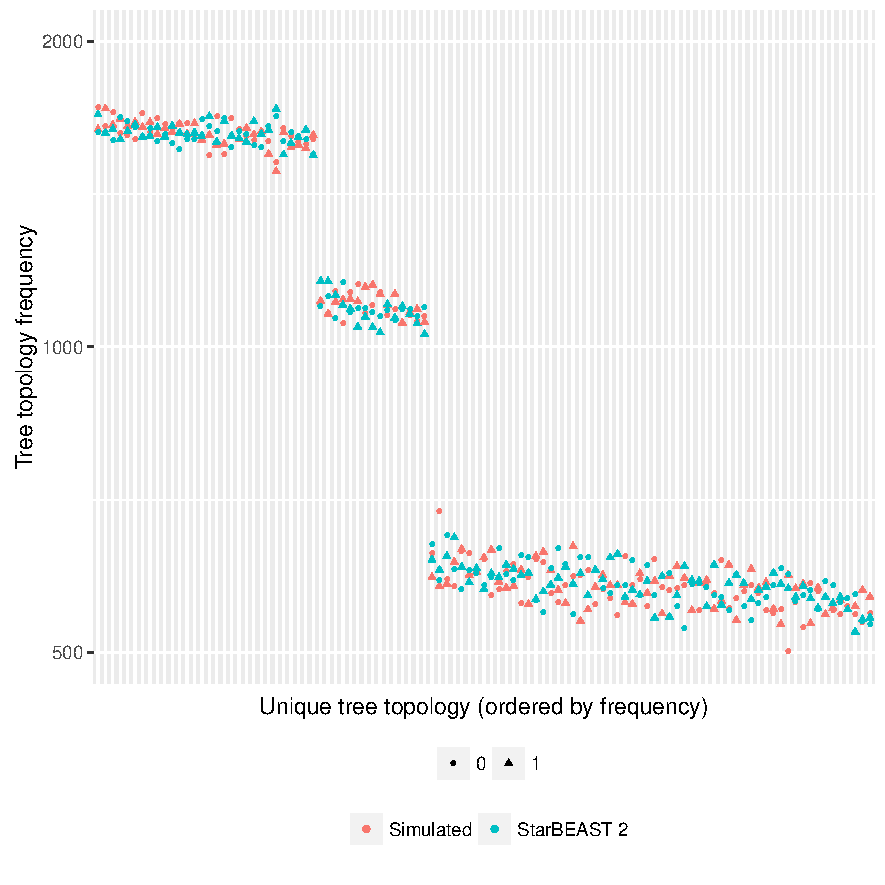
\includegraphics[width=16cm]{gene_topology_frequencies.pdf}
\caption
{bbb.}
\label{fig:geneTopologyFrequencies}
\end{figure}

\clearpage

\begin{figure}[htb!]
\centering
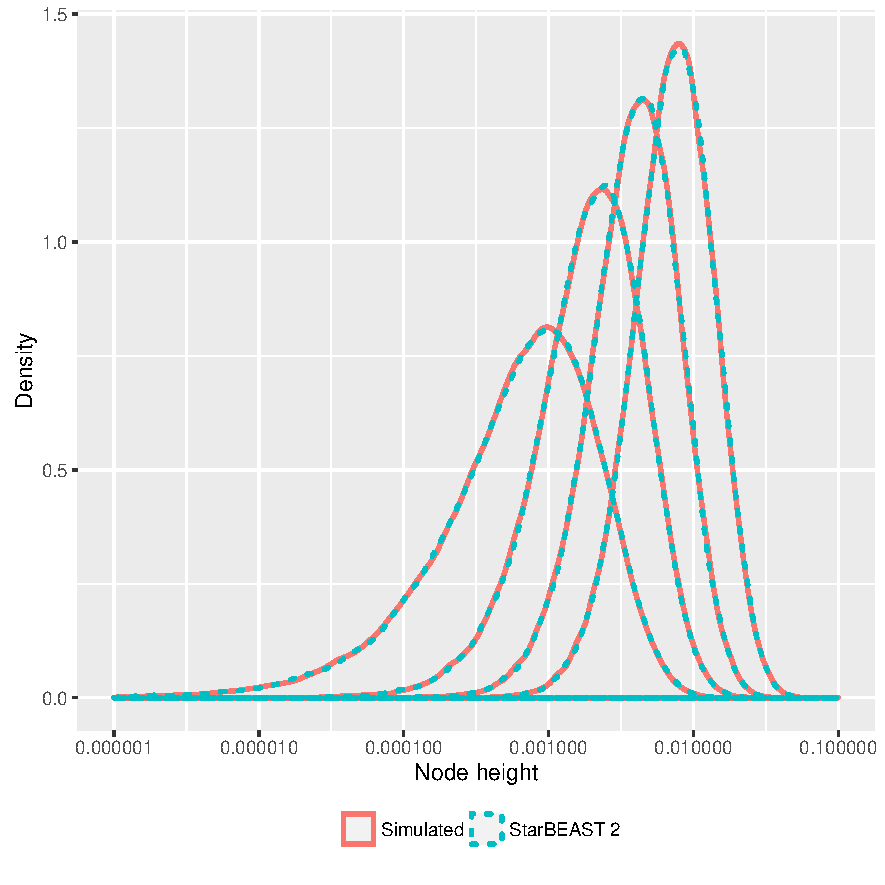
\includegraphics[width=16cm]{species_node_heights.pdf}
\caption
{ccc.}
\label{fig:speciesNodeHeights}
\end{figure}

\clearpage

\begin{figure}[htb!]
\centering
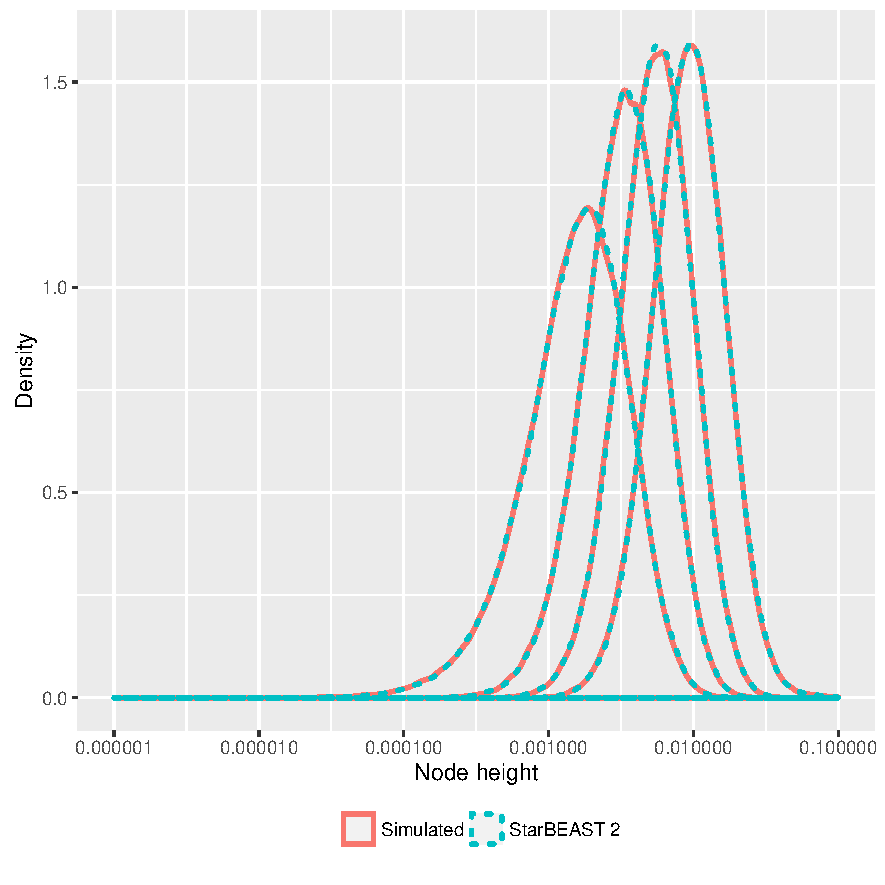
\includegraphics[width=16cm]{gene_node_heights.pdf}
\caption
{ddd.}
\label{fig:geneNodeHeights}
\end{figure}

\clearpage

\begin{figure}[htb!]
\centering
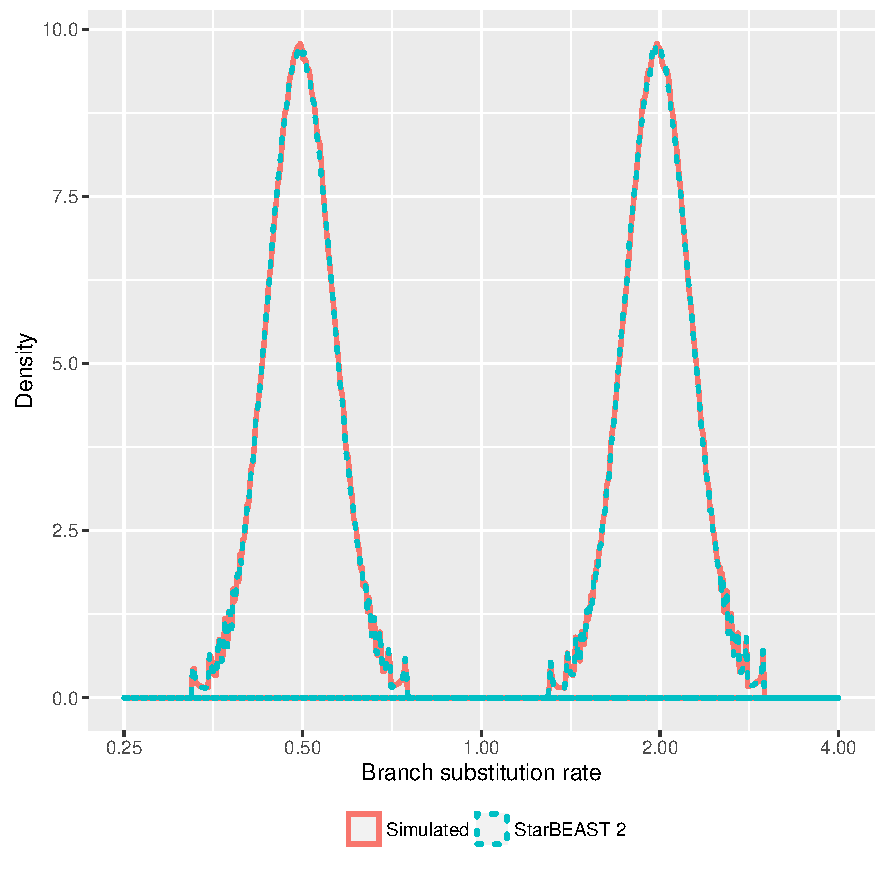
\includegraphics[width=16cm]{gene_branch_rates.pdf}
\caption
{eee.}
\label{fig:geneBranchRates}
\end{figure}

\clearpage

\end{document}
